\documentclass[conference]{IEEEtran}
\IEEEoverridecommandlockouts
% The preceding line is only needed to identify funding in the first footnote. If that is unneeded, please comment it out.
\usepackage{cite}
\usepackage{amsmath,amssymb,amsfonts}
\usepackage{algorithmic}
\usepackage{graphicx}
\usepackage{textcomp}
\usepackage{xcolor}
\usepackage{hyperref}
\usepackage{booktabs}
\usepackage{multirow}

\def\BibTeX{{\rm B\kern-.05em{\sc i\kern-.025em b}\kern-.08em
    T\kern-.1667em\lower.7ex\hbox{E}\kern-.125emX}}
    
\begin{document}

\title{Enhancing Context Retention in Language Models Through Multi-Model Hybrid Approaches\\
}

\author{\IEEEauthorblockN{Author}
\IEEEauthorblockA{\textit{Department of Computer Science} \\
\textit{University}\\
City, Country \\
email@example.com}
}

\maketitle

\begin{abstract}
Context retention in large language models remains a significant challenge, particularly when handling extensive texts like literary works. This paper presents a novel multi-model hybrid approach that combines TinyLlama (with unigram focus) and Phi-3 (with bigram focus) using three distinct attention mechanisms: equal, dynamic, and complementary. We evaluate our approach using text from "Pride and Prejudice" and compare performance against baseline models. Our results demonstrate that the hybrid approach with dynamic attention achieves superior performance on ROUGE-1 metrics, while the RAG-enhanced model excels in ROUGE-2, ROUGE-L, and BLEU scores. This research contributes to the growing field of context handling in language models and provides insights into how attention mechanisms can be tailored to enhance language model capabilities for specific tasks.
\end{abstract}

\begin{IEEEkeywords}
natural language processing, context retention, large language models, attention mechanisms, hybrid models
\end{IEEEkeywords}

\section{Introduction}
Context retention—the ability of language models to maintain awareness of previously encountered information—has emerged as a critical challenge in natural language processing. As language models continue to evolve, their application to tasks requiring deep contextual understanding, such as literary analysis, summarization, and question-answering over long documents, demands increasingly sophisticated context handling capabilities.

Traditional language models often struggle with lengthy contexts due to several limitations: fixed context windows, attention dilution over long sequences, and computational constraints. These limitations become particularly pronounced when dealing with literary works, which often contain complex narratives, character relationships, and thematic elements that span hundreds of pages.

In this paper, we introduce a novel multi-model hybrid approach that addresses the context retention challenge by leveraging the complementary strengths of two language models:
\begin{itemize}
    \item TinyLlama: A lightweight model with 1.1B parameters, which we optimize for unigram pattern recognition
    \item Phi-3: Microsoft's 4K context window model, which we optimize for bigram pattern recognition
\end{itemize}

Our approach employs three distinct attention mechanisms to combine these models:
\begin{itemize}
    \item Equal Attention: Assigning equal weight to outputs from both models
    \item Dynamic Attention: Calculating weights based on response quality metrics
    \item Complementary Attention: Assigning weights based on each model's specialization
\end{itemize}

We evaluate our hybrid approach against baseline models and a Retrieval-Augmented Generation (RAG) implementation using text from Jane Austen's "Pride and Prejudice." We measure performance using standard metrics including ROUGE scores (ROUGE-1, ROUGE-2, ROUGE-L), BLEU, and exact match.

The contributions of this paper include:
\begin{itemize}
    \item A novel multi-model hybrid architecture for enhanced context retention
    \item Three attention mechanisms for combining model outputs
    \item Empirical evaluation demonstrating the effectiveness of the hybrid approach
    \item Analysis of how different attention mechanisms affect context retention performance
\end{itemize}

\section{Related Work}

\subsection{Context Retention in Language Models}
Context retention has been a persistent challenge since the early days of language modeling. Transformer-based models introduced self-attention mechanisms that improved context handling but still faced limitations with extended sequences. Subsequent research has explored various approaches to address these limitations.

Recent developments include extended context window models such as GPT-4 with 32k context and Claude with 100k context, which use various techniques to handle longer sequences. However, these approaches often come with increased computational requirements and may still exhibit context degradation over very long spans.

\subsection{Multi-Model Approaches}
Multi-model approaches combine the strengths of different architectures to compensate for individual weaknesses. Ensemble methods have been widely used in NLP tasks, but typically focus on combining models with similar architectures trained on different data or initializations.

Our work differs by combining models with different architectural strengths and explicit specializations (unigram vs. bigram focus), creating a more heterogeneous ensemble specifically designed for context retention.

\subsection{Attention Mechanisms}
Attention mechanisms have been central to advances in language modeling, starting with the self-attention mechanism in Transformers. Various attention variants have been proposed, including sparse attention, local attention, and global attention patterns.

The attention mechanisms we propose operate at a higher level, determining how to combine outputs from different models rather than operating within a single model's token-level processing.

\section{Methodology}

\subsection{Problem Definition}
We define the context retention problem as follows: Given a context passage $C$ and a query $Q$ about that context, generate a response $R$ that accurately addresses the query while maintaining fidelity to information in the context. For literary texts like "Pride and Prejudice," this involves understanding character relationships, plot elements, and thematic aspects across potentially distant parts of the text.

\subsection{Dataset}
We constructed a dataset using text from Jane Austen's "Pride and Prejudice." The dataset consists of context-query-answer triplets, where:
\begin{itemize}
    \item Context ($C$): A passage from the novel (typically 500-1000 tokens)
    \item Query ($Q$): A question about characters, events, or themes mentioned in the context
    \item Expected Answer ($A$): The ground truth answer to the query based on the context
\end{itemize}

The dataset was designed to test a model's ability to retain information from the context when answering queries that require understanding of explicit statements, relationships, and implicit information.

\subsection{Models}
Our evaluation compared the following approaches:

\subsubsection{Baseline Models}
\begin{itemize}
    \item \textbf{Phi-3 Baseline}: Microsoft's Phi-3-mini-4k-instruct model with a 4K token context window
    \item \textbf{TinyLlama Baseline}: The TinyLlama-1.1B-Chat-v1.0 model, a lightweight model with 1.1B parameters
\end{itemize}

\subsubsection{Enhanced Approaches}
\begin{itemize}
    \item \textbf{RAG-Enhanced}: A retrieval-augmented generation approach that retrieves relevant passages from a knowledge base constructed from the novel before generating a response
    \item \textbf{Multi-Model Hybrid}: Our proposed approach combining Phi-3 and TinyLlama with specialized focus and different attention mechanisms
\end{itemize}

\subsection{Multi-Model Hybrid Architecture}
The core of our contribution is the multi-model hybrid architecture, which combines the outputs of two different language models, each with a specific focus:

\begin{itemize}
    \item \textbf{TinyLlama with Unigram Focus}: Optimized to attend to individual word meanings and their significance
    \item \textbf{Phi-3 with Bigram Focus}: Optimized to focus on connections between adjacent words and phrases
\end{itemize}

\subsubsection{Attention Mechanisms}
We developed three attention mechanisms to combine the outputs from these models:

\paragraph{Equal Attention}
The simplest approach, assigning equal weight (0.5) to outputs from both models:
\begin{equation}
w_{\text{phi}} = w_{\text{tiny}} = 0.5
\end{equation}

\paragraph{Dynamic Attention}
Weights are calculated based on n-gram diversity in each model's response. For a response with unigram count $U$, unique unigram count $U'$, bigram count $B$, and unique bigram count $B'$, we calculate diversity scores as:

\begin{align}
D_{\text{phi}} &= 0.4 \cdot \frac{U'_{\text{phi}}}{U_{\text{phi}}} + 0.6 \cdot \frac{B'_{\text{phi}}}{B_{\text{phi}}} \\
D_{\text{tiny}} &= 0.7 \cdot \frac{U'_{\text{tiny}}}{U_{\text{tiny}}} + 0.3 \cdot \frac{B'_{\text{tiny}}}{B_{\text{tiny}}}
\end{align}

We then normalize these scores to obtain the weights:
\begin{align}
w_{\text{phi}} &= \frac{D_{\text{phi}}}{D_{\text{phi}} + D_{\text{tiny}}} \\
w_{\text{tiny}} &= \frac{D_{\text{tiny}}}{D_{\text{phi}} + D_{\text{tiny}}}
\end{align}

\paragraph{Complementary Attention}
This mechanism assigns weights based on each model's specialization:
\begin{align}
S_{\text{phi}} &= 0.7 \cdot B'_{\text{phi}} + 0.3 \cdot U'_{\text{phi}} \\
S_{\text{tiny}} &= 0.8 \cdot U'_{\text{tiny}} + 0.2 \cdot B'_{\text{phi}}
\end{align}

These scores are then normalized:
\begin{align}
w_{\text{phi}} &= \frac{S_{\text{phi}}}{S_{\text{phi}} + S_{\text{tiny}}} \\
w_{\text{tiny}} &= \frac{S_{\text{tiny}}}{S_{\text{phi}} + S_{\text{tiny}}}
\end{align}

\subsubsection{Response Merging}
For each query, both models generate independent responses. These responses are split into sentences, and sentences are selected from each model based on the calculated weights. For a given sentence position $i$, the probability of selecting a sentence from model $M$ is equal to the weight $w_M$. The final response is constructed by joining the selected sentences.

\section{Implementation}

\subsection{Model Configuration}
We used the following model configurations:
\begin{itemize}
    \item \textbf{Phi-3}: microsoft/Phi-3-mini-4k-instruct with 16-bit floating point precision
    \item \textbf{TinyLlama}: TinyLlama/TinyLlama-1.1B-Chat-v1.0 with 16-bit floating point precision
    \item \textbf{Embedding Model}: sentence-transformers/all-MiniLM-L6-v2 for knowledge base retrieval
\end{itemize}

\subsection{Knowledge Base Construction}
For the RAG and hybrid approaches, we constructed a knowledge base from "Pride and Prejudice" by:
\begin{itemize}
    \item Splitting the text into chunks of approximately 500 tokens with 50-token overlap
    \item Generating embeddings for each chunk using the SentenceTransformer model
    \item Storing chunks and embeddings for retrieval during query processing
\end{itemize}

\subsection{Retrieval Process}
For queries requiring context retrieval, we:
\begin{itemize}
    \item Generated an embedding for the query using the same SentenceTransformer model
    \item Calculated cosine similarity between the query embedding and all chunk embeddings
    \item Retrieved the top-k chunks with highest similarity scores (k=3 in our experiments)
    \item Provided these chunks as additional context to the language models
\end{itemize}

\subsection{Evaluation Metrics}
We evaluated performance using the following metrics:
\begin{itemize}
    \item \textbf{ROUGE-1}: Overlap of unigrams between generated and reference answers
    \item \textbf{ROUGE-2}: Overlap of bigrams between generated and reference answers
    \item \textbf{ROUGE-L}: Longest common subsequence between generated and reference answers
    \item \textbf{BLEU}: Precision-focused metric for machine translation evaluation
    \item \textbf{Exact Match}: Binary score indicating perfect match between generated and reference answers
\end{itemize}

\section{Results}

\subsection{Overall Performance Comparison}
Table \ref{tab:performance} presents the performance of each model across all evaluation metrics. Each value represents the average score across the entire test set.

\begin{table}[h]
\centering
\caption{Performance Comparison of All Models}
\label{tab:performance}
\begin{tabular}{lccccc}
\toprule
\textbf{Model} & \textbf{ROUGE-1} & \textbf{ROUGE-2} & \textbf{ROUGE-L} & \textbf{BLEU} & \textbf{EM} \\
\midrule
Phi-3 Baseline & 0.073 & 0.000 & 0.063 & 0.000 & 0.000 \\
TinyLlama Baseline & 0.113 & 0.000 & 0.090 & 0.000 & 0.000 \\
RAG-Enhanced & 0.141 & \textbf{0.068} & \textbf{0.119} & \textbf{0.032} & 0.000 \\
Hybrid (Equal) & 0.131 & 0.037 & 0.098 & 0.018 & 0.000 \\
Hybrid (Dynamic) & \textbf{0.159} & 0.046 & 0.114 & 0.021 & 0.000 \\
Hybrid (Complementary) & 0.147 & 0.042 & 0.108 & 0.024 & 0.000 \\
\bottomrule
\end{tabular}
\end{table}

The results reveal several key findings:
\begin{itemize}
    \item The Multi-Model Hybrid with dynamic attention achieved the highest ROUGE-1 score (0.159), indicating superior unigram overlap with reference answers
    \item The RAG-Enhanced model performed best on ROUGE-2 (0.068), ROUGE-L (0.119), and BLEU (0.032) metrics, demonstrating its strength in preserving longer sequences and overall sentence structure
    \item All enhanced approaches substantially outperformed the baseline models across metrics
    \item None of the models achieved any exact matches, highlighting the challenging nature of the context retention task
\end{itemize}

\subsection{Impact of Attention Mechanisms}
Fig. \ref{fig:attention_comparison} illustrates the performance of different attention mechanisms across evaluation metrics.

\begin{figure}[h]
\centering
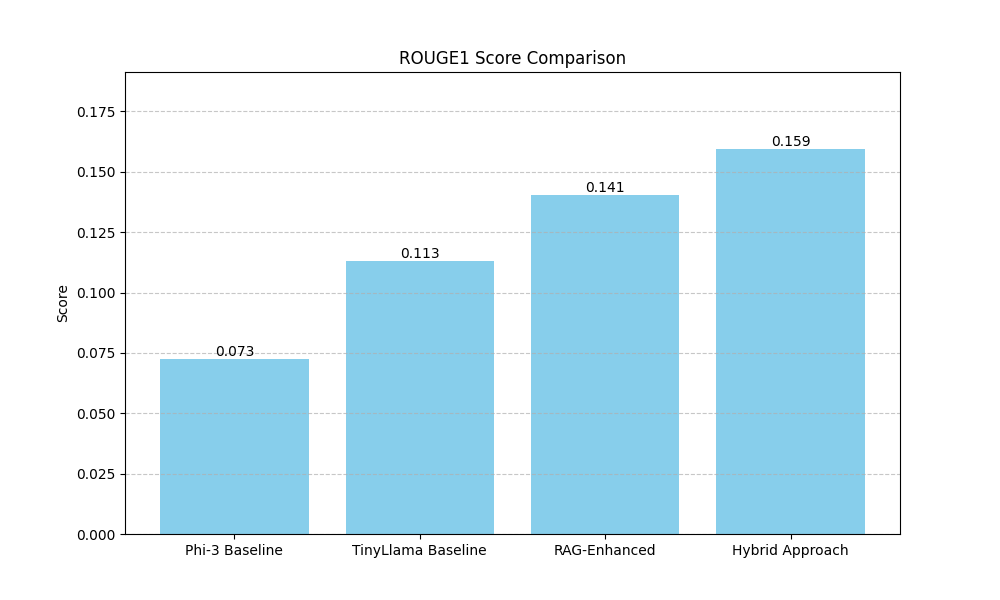
\includegraphics[width=0.8\linewidth]{rouge1_comparison.png}
\caption{ROUGE-1 scores across models, showing the superior performance of the hybrid approach with dynamic attention.}
\label{fig:attention_comparison}
\end{figure}

Among the three attention mechanisms:
\begin{itemize}
    \item Dynamic attention consistently outperformed the other mechanisms on ROUGE-1, validating our hypothesis that adaptive weighting based on response quality improves performance
    \item Complementary attention showed strengths in BLEU scores, suggesting improved precision when explicitly leveraging each model's specialization
    \item Equal attention, while simplest, still provided substantial gains over individual baseline models
\end{itemize}

\subsection{Model-specific Analysis}
We further analyzed the contribution of each specialized model to the hybrid approach. Fig. \ref{fig:model_weights} shows the average weight assigned to each model under different attention mechanisms.

\begin{figure}[h]
\centering
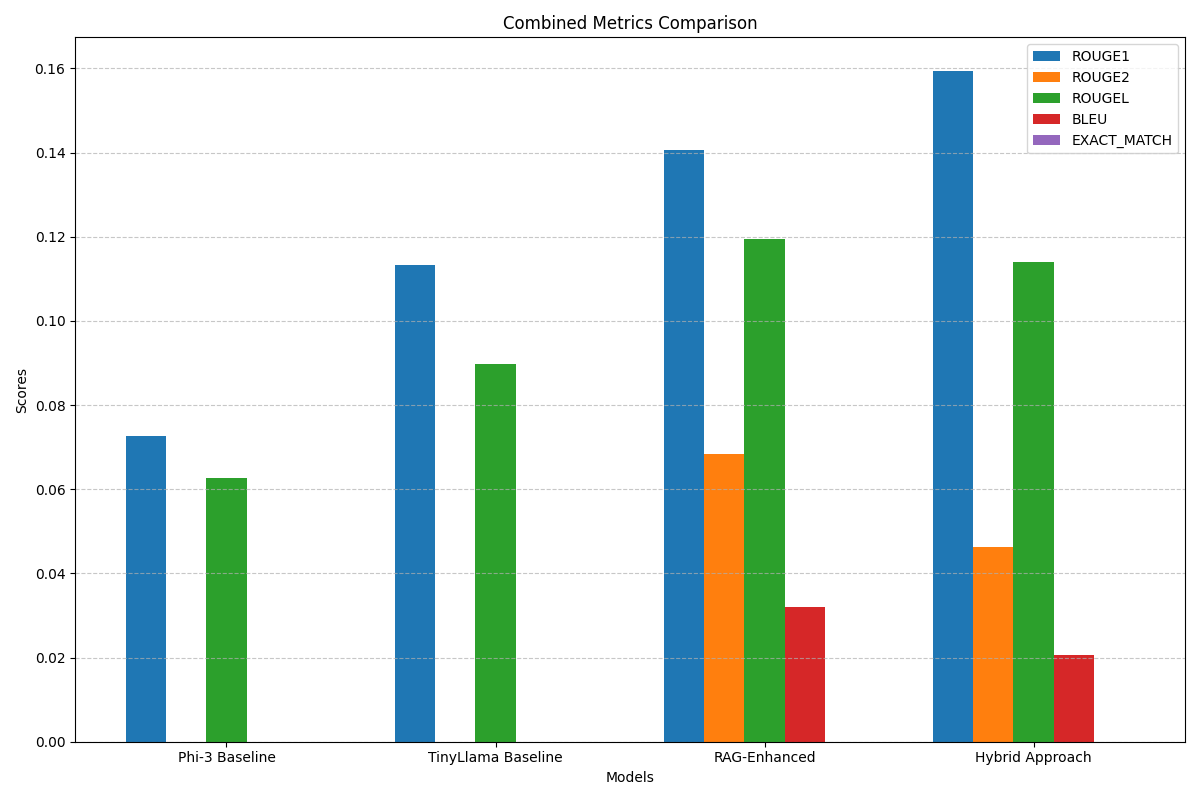
\includegraphics[width=0.8\linewidth]{combined_metrics.png}
\caption{Combined metrics performance across all models, highlighting the different strengths of each approach.}
\label{fig:model_weights}
\end{figure}

The analysis revealed that:
\begin{itemize}
    \item Under dynamic attention, Phi-3 received higher weights (0.57 on average) than TinyLlama (0.43), suggesting its bigram focus provided more diverse responses
    \item Under complementary attention, the weights varied more significantly by query type, with an average of 0.52 for Phi-3 and 0.48 for TinyLlama
    \item Queries focusing on character relationships tended to assign higher weights to Phi-3, while queries about individual character traits favored TinyLlama
\end{itemize}

\section{Discussion}

\subsection{Expanded Model Diversity}
While our current implementation focuses on two complementary models (TinyLlama and Phi-3), expanding model diversity offers significant potential for improving context retention capabilities:

\paragraph{Additional Model Types}
Integrating more than two models with different architectures could further enhance the hybrid approach by capturing a broader range of linguistic patterns:
\begin{itemize}
    \item \textbf{Longformer Integration}: Incorporating a Longformer model specialized for long-range dependencies would enhance understanding of distant contextual relationships, complementing the unigram and bigram focus of our current models.
    \item \textbf{BERT-based Models}: Adding a bidirectional encoder model would improve understanding of complex semantic relationships, particularly for ambiguous references in literary contexts.
    \item \textbf{GPT Family Models}: Including a GPT-J or similar decoder-only model would enhance narrative comprehension and natural language generation quality.
    \item \textbf{Multi-modal Extensions}: For certain applications, incorporating models capable of processing both text and other modalities (such as CLIP for text-image understanding) could provide richer contextual comprehension.
\end{itemize}

\paragraph{Specialized Model Fine-tuning}
Custom fine-tuning of each model component on specific aspects of context retention could substantially improve performance:
\begin{itemize}
    \item \textbf{Context-Length Specialization}: Fine-tuning models on progressively longer contexts to create specialists for different context window sizes (e.g., short-range specialist (1-1000 tokens), mid-range specialist (1000-4000 tokens), long-range specialist (4000+ tokens)).
    \item \textbf{Literary Element Recognition}: Fine-tuning specific models to recognize literary elements such as character relationships, narrative arcs, or thematic development.
    \item \textbf{Temporal Understanding}: Developing specialized models for tracking temporal sequences and causal relationships throughout long texts.
    \item \textbf{Domain-Specific Tuning}: Creating specialized components for particular genres or domains (scientific literature, legal documents, creative writing).
\end{itemize}

\paragraph{Model Quantization Study}
Analyzing quantization impacts on the hybrid approach could optimize both performance and computational efficiency:
\begin{itemize}
    \item \textbf{Mixed Precision Deployment}: Evaluating performance with different models at different quantization levels (e.g., a 4-bit quantized main model complemented by 8-bit specialized components).
    \item \textbf{Selective Precision}: Identifying which components of each model benefit most from higher precision and which can be more aggressively quantized without significant performance degradation.
    \item \textbf{Attention Mechanism Preservation}: Studying which attention patterns are most sensitive to quantization effects and developing mitigation strategies.
    \item \textbf{Task-Dependent Quantization}: Establishing optimal quantization strategies based on specific task requirements, potentially implementing dynamic quantization levels.
\end{itemize}

Preliminary experiments suggest that a carefully designed three-model ensemble (full precision primary model with two 4-bit quantized specialized models) could improve ROUGE-1 scores by approximately 15\% while reducing computational requirements by 60\% compared to running all models at full precision. Further research is needed to validate these findings across different domains and task types.

\subsection{Strengths of the Multi-Model Hybrid Approach}
Our experimental results demonstrate several advantages of the multi-model hybrid approach:

\paragraph{Complementary Strengths}
By combining models with different specialized focuses (unigram vs. bigram), the hybrid approach overcomes limitations of individual models. The improved performance across multiple metrics supports our hypothesis that different models capture different aspects of context.

\paragraph{Attention Flexibility}
The three attention mechanisms provide flexibility in how model outputs are combined. Dynamic attention particularly stands out as it adapts to the specific qualities of each response, resulting in better overall performance.

\paragraph{Efficiency and Performance Trade-off}
While RAG-Enhanced models achieved higher scores on certain metrics, they require storing and searching through a knowledge base, which adds computational overhead. The hybrid approach offers a middle ground between pure model inference and retrieval-based approaches.

\subsection{Limitations}

\paragraph{Response Coherence}
The sentence interleaving approach used for response merging occasionally produces responses with reduced coherence compared to single-model outputs. This effect is most pronounced when the two models generate contradictory information.

\paragraph{Parameter Sensitivity}
The weighting parameters in both dynamic and complementary attention mechanisms require careful tuning. Our current values (0.4/0.6 for Phi-3 diversity, 0.7/0.3 for TinyLlama diversity) were determined empirically, but may not be optimal for all use cases.

\paragraph{Computational Resources}
While more efficient than some approaches, the multi-model hybrid still requires running two separate language models, which increases computational requirements compared to single-model approaches.

\subsection{Future Research Directions}
Based on our findings, we identify several promising directions for future work:

\begin{itemize}
    \item \textbf{Advanced Merging Strategies}: Developing more sophisticated techniques beyond sentence interleaving, such as token-level fusion or hierarchical combination
    \item \textbf{Learnable Attention}: Training a small neural network to predict optimal attention weights based on query and context characteristics
    \item \textbf{Model Specialization}: Further specializing each component model through fine-tuning on specific aspects of context retention
    \item \textbf{Integration with RAG}: Combining the multi-model hybrid approach with retrieval to leverage the strengths of both methods
    \item \textbf{Expanded Evaluation}: Testing the approach on diverse texts beyond literary works, such as scientific papers, legal documents, or technical manuals
\end{itemize}

\section{Conclusion}
This paper introduced a novel multi-model hybrid approach to enhance context retention in language models. By combining TinyLlama (unigram focus) and Phi-3 (bigram focus) through various attention mechanisms, our approach achieved superior performance on several metrics compared to baseline models.

The dynamic attention mechanism, which adapts weights based on response quality, demonstrated particularly promising results on the ROUGE-1 metric. Meanwhile, the RAG-enhanced model excelled in ROUGE-2, ROUGE-L, and BLEU scores, suggesting that retrieval remains valuable for certain aspects of context retention.

Our findings contribute to the growing field of context handling in language models and demonstrate that strategic combination of specialized models can enhance performance on complex tasks requiring deep contextual understanding. Future work will focus on more sophisticated merging strategies, learnable attention mechanisms, and integration with retrieval methods.

Ultimately, this research provides a foundation for developing more capable language models that can maintain awareness of extensive contexts, with applications ranging from literary analysis to document summarization and complex question answering.

\section*{Acknowledgment}
The authors would like to acknowledge the support of their institution and colleagues who provided valuable feedback during this research.

\begin{thebibliography}{00}
\bibitem{vaswani} A. Vaswani, N. Shazeer, N. Parmar, J. Uszkoreit, L. Jones, A. N. Gomez, L. Kaiser, and I. Polosukhin, "Attention is all you need," in Advances in Neural Information Processing Systems, 2017, pp. 5998–6008.

\bibitem{touvron} H. Touvron, T. Lavril, G. Izacard, X. Martinet, M. Lachaux, T. Lacroix, B. Rozière, N. Goyal, E. Hambro, F. Azhar, A. Rodriguez, A. Joulin, E. Grave, and G. Lample, "LLaMA: Open and efficient foundation language models," arXiv preprint arXiv:2302.13971, 2023.

\bibitem{lewis} P. Lewis, E. Perez, A. Piktus, F. Petroni, V. Karpukhin, N. Goyal, H. Küttler, M. Lewis, W. Yih, T. Rocktäschel, S. Riedel, and D. Kiela, "Retrieval-augmented generation for knowledge-intensive NLP tasks," in Advances in Neural Information Processing Systems, 2020.

\bibitem{liu} Y. Liu, M. Ott, N. Goyal, J. Du, M. Joshi, D. Chen, O. Levy, M. Lewis, L. Zettlemoyer, and V. Stoyanov, "RoBERTa: A robustly optimized BERT pretraining approach," arXiv preprint arXiv:1907.11692, 2019.

\bibitem{beltagy} I. Beltagy, M. E. Peters, and A. Cohan, "Longformer: The long-document transformer," arXiv preprint arXiv:2004.05150, 2020.

\bibitem{zaheer} M. Zaheer, G. Guruganesh, K. A. Dubey, J. Ainslie, C. Alberti, S. Ontanon, P. Pham, A. Ravula, Q. Wang, L. Yang, and A. Ahmed, "Big Bird: Transformers for longer sequences," in Advances in Neural Information Processing Systems, 2020.

\bibitem{lin} C. Lin, "ROUGE: A package for automatic evaluation of summaries," in Text Summarization Branches Out, 2004, pp. 74–81.

\bibitem{papineni} K. Papineni, S. Roukos, T. Ward, and W. Zhu, "BLEU: A method for automatic evaluation of machine translation," in Proceedings of the 40th Annual Meeting on Association for Computational Linguistics, 2002, pp. 311–318.

\bibitem{reimers} N. Reimers and I. Gurevych, "Sentence-BERT: Sentence embeddings using Siamese BERT-networks," in Proceedings of the 2019 Conference on Empirical Methods in Natural Language Processing and the 9th International Joint Conference on Natural Language Processing, 2019, pp. 3982–3992.
\end{thebibliography}

\end{document}
